%!TeX root = Dissertation-DonaldDuck.tex
%!TEX TS-program = Arara
% arara: pdflatex: {shell: yes}
% arara: pdflatex: {shell: yes}
\chapter{Fazit}\label{cha:Fazit}

\blindtext[5]

\begin{figure}
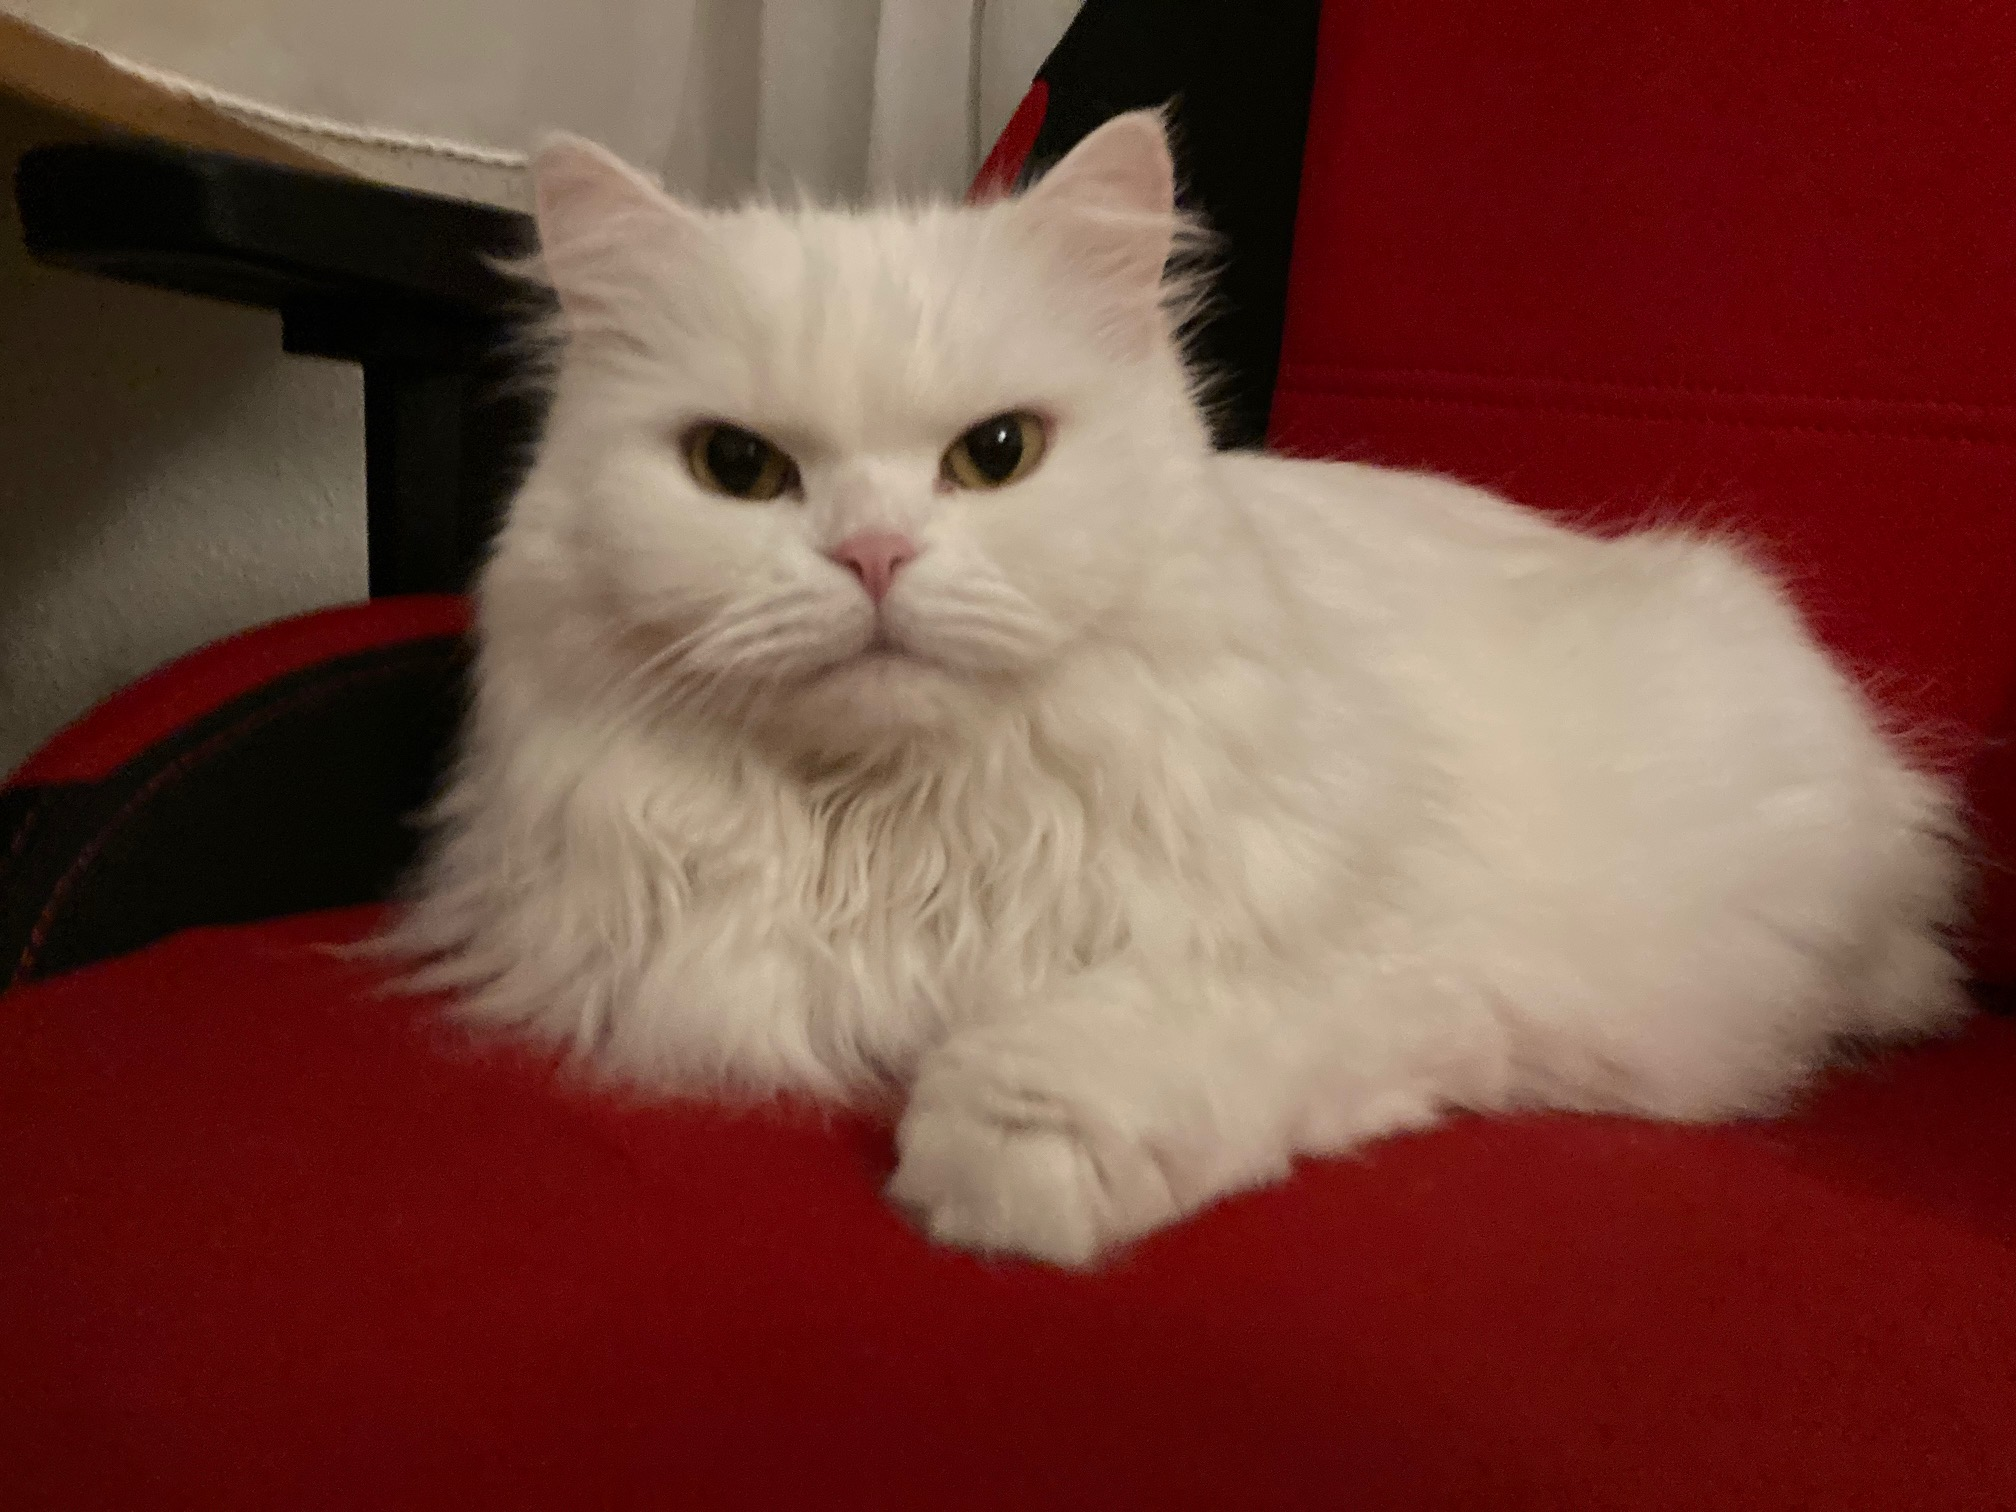
\includegraphics[width=\textwidth]{Bilder/Katze}
\caption{Meine Katze}\label{fig:Katze}
\end{figure}

\blindtext[5]

% Alternative zum Float
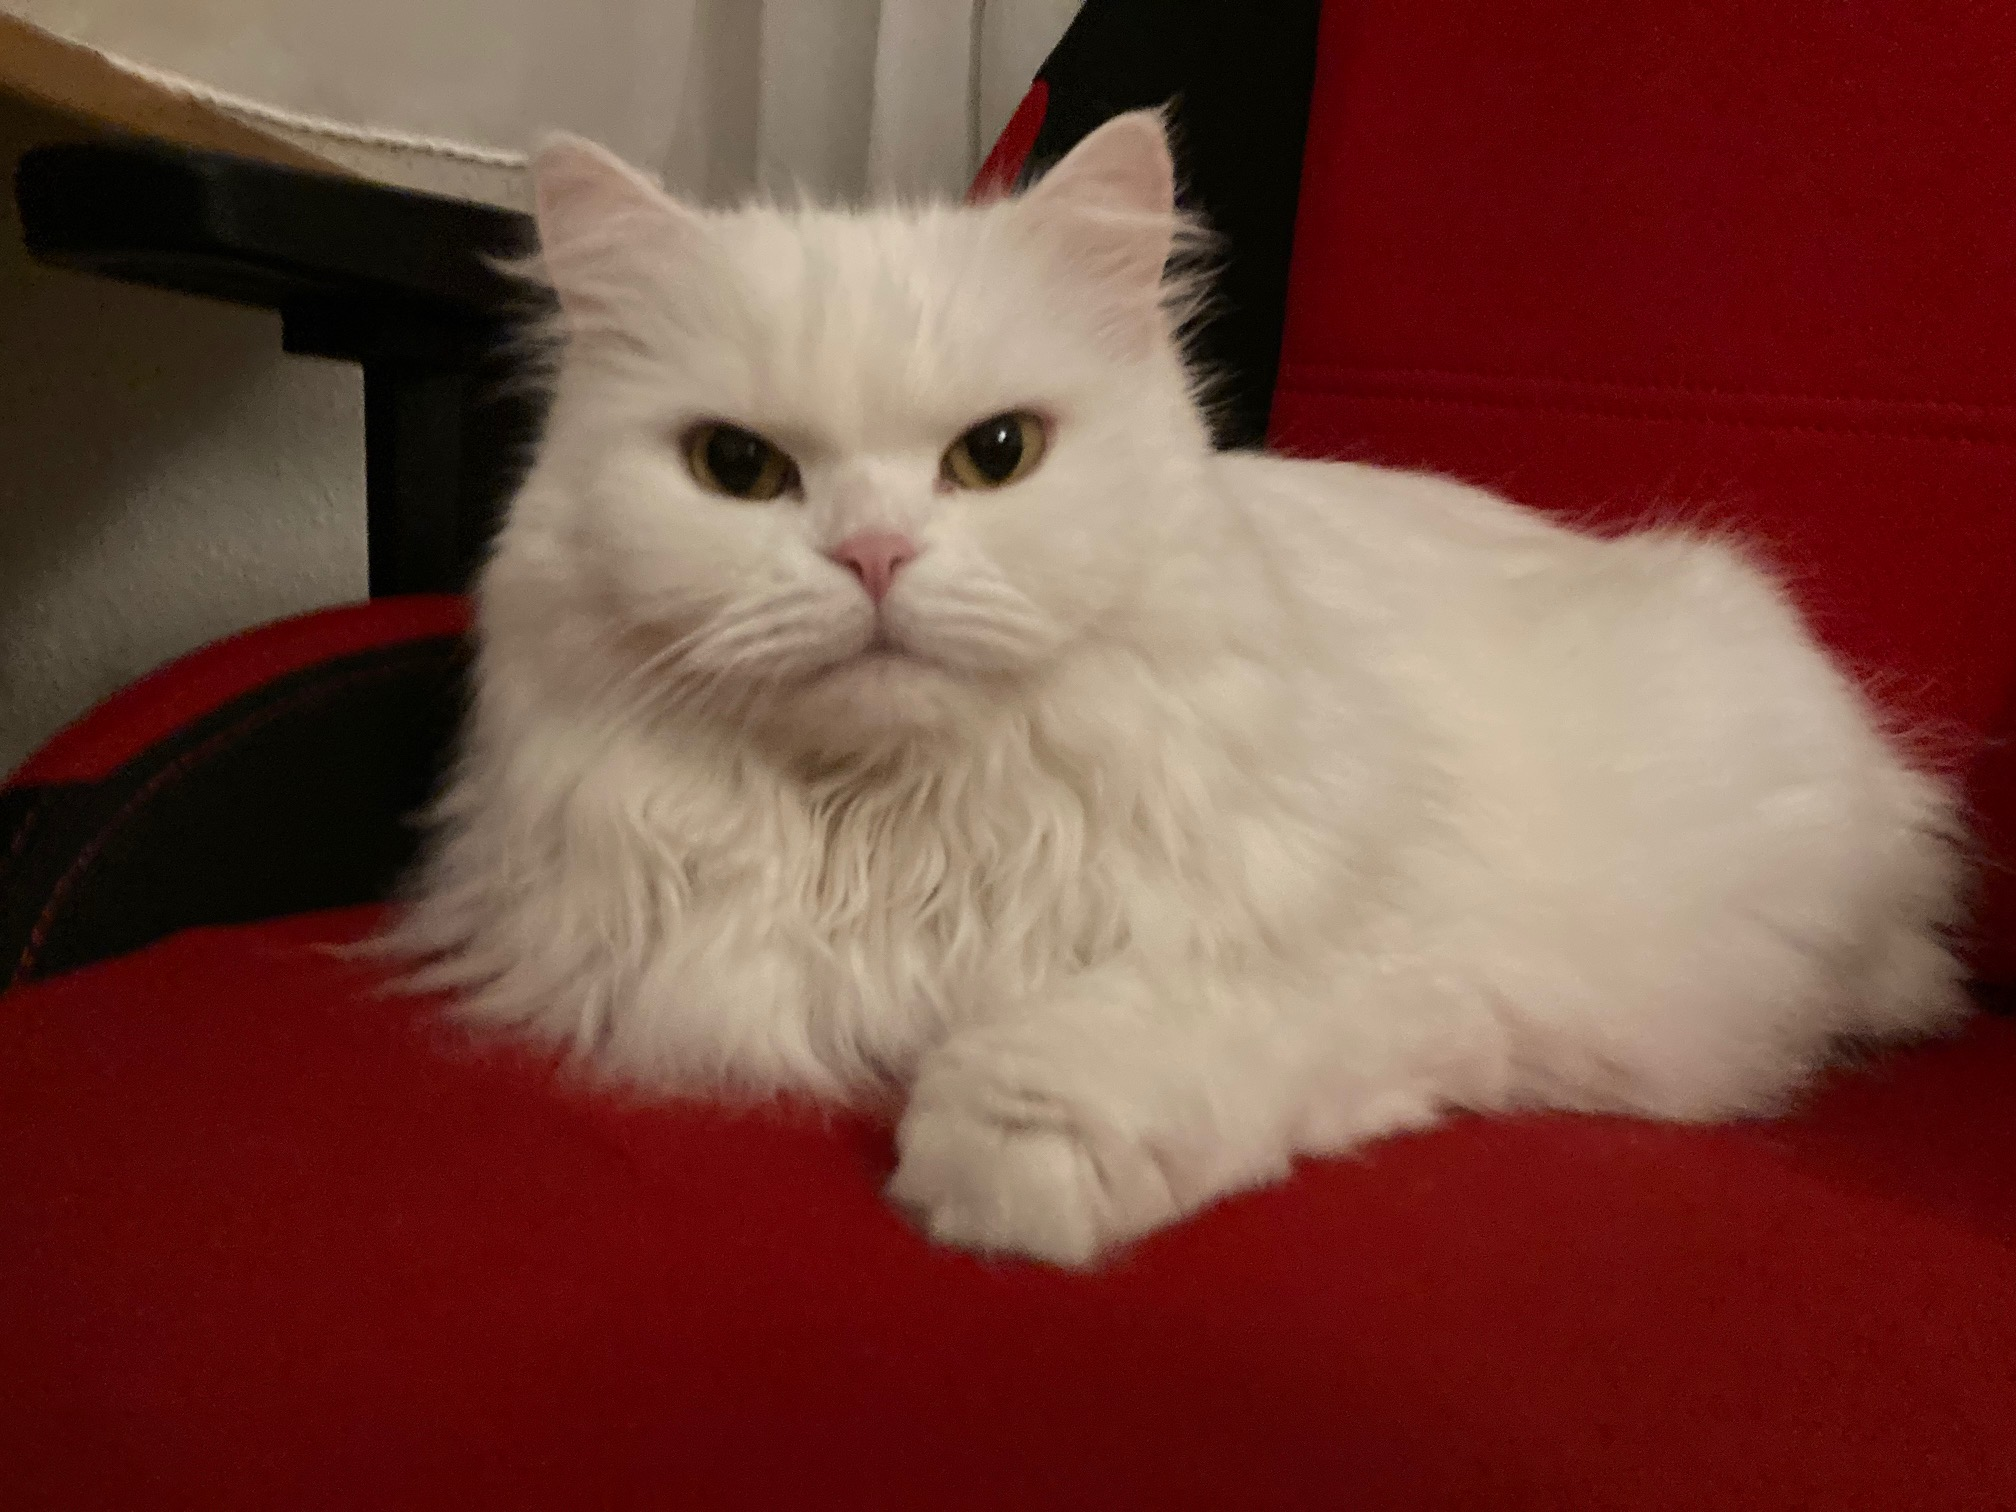
\includegraphics[width=\textwidth]{Bilder/Katze}
\captionof{figure}{Meine Katze 2}\label{fig:Katze2}

\blindtext[12]

\blindtext \cite{Knuth1984}, \cite{Knuth1984}  and \cite{Buchin2023} have shown, that elliptic curves are useful in computing. \cite{Yu2021} also showed this   .\footnote{\blindtext}

\cite{Ziegenhagen2022}

parencite \parencite{Knuth1984}

Uwe Ziegenhagen\footcite{Ziegenhagen2022}

citeauthor, citetitle und citeyear kombiniert: \citeauthor{Knuth1984} hat in seinem im Jahre \citeyear{Knuth1984} erschienenen Buch \citetitle{Knuth1984} bewiesen, dass \(p = np \)

\printbibliography[title={Bücher},type=book] 

\printbibliography[title={Artikel},type=article] 

\printbibliography[title={Online-Quellen},type=www] 

